\documentclass[12pt]{article}
\usepackage{amsmath, amssymb}
\usepackage{enumitem}
\usepackage{graphicx}
\usepackage[margin=1in]{geometry}

% Custom macro as per your preference
\newcommand{\myvec}[1]{\begin{bmatrix}#1\end{bmatrix}}

\begin{document}

\begin{center}
    {\LARGE \bf GATE -MT 2019}\\[1em]
    ai25btech11009 \quad Dasu Harshith Kumar
\end{center}

\begin{enumerate}

\item One of the eigenvalues for the following matrix is \hspace{1em} (GATE 2019 MT)
\[
\myvec{a & 2 \\
       8 & a}
\]
\begin{enumerate}[label=(\alph*)]
    \item $a-4$
    \item $-a-4$
    \item $4$
    \item $-4$
\end{enumerate}

\item The curl of vector fields shown below is not zero for \hspace{1em} (GATE 2019 MT)
\begin{center}
    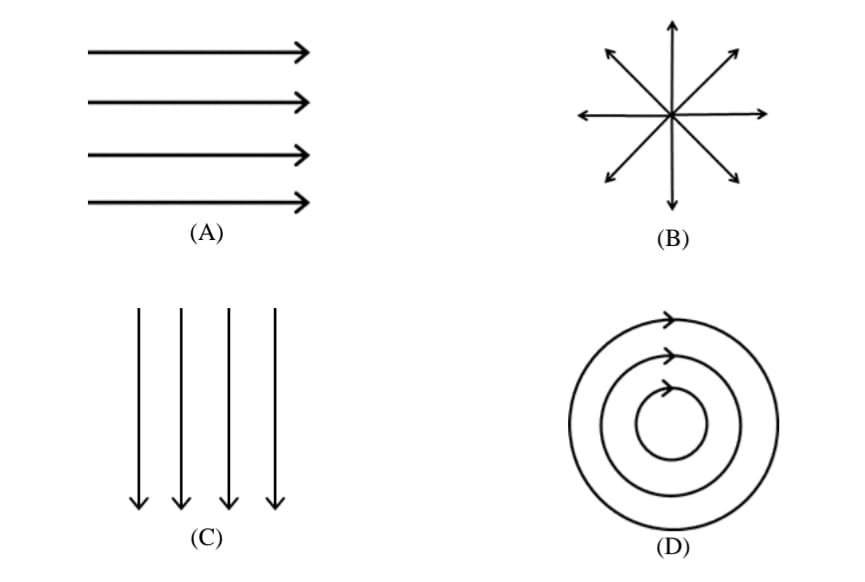
\includegraphics[width=0.9\textwidth]{images/qq2oi.jpg}
\end{center}
% Option image should show all vector field diagrams

\item The smallest period of the function $f(x) = \sin\left(\frac{n x}{k}\right)$ is \hspace{1em} (GATE 2019 MT)
\begin{enumerate}[label=(\alph*)]
    \item $2\pi$
    \item $\dfrac{k}{n}$
    \item $\dfrac{2\pi k}{n}$
    \item $\dfrac{2\pi n}{k}$
\end{enumerate}

\item The directional derivative of $\phi = x^2 + y$ along unit vector $\vec{u} = \frac{1}{5}(3\hat{i} + 4\hat{j})$ at $(1,1)$ is \hspace{1em} (GATE 2019 MT)
\begin{enumerate}[label=(\alph*)]
    \item 3
    \item 2
    \item 1
    \item 0
\end{enumerate}

\item Liquid steel is kept in a graphite crucible for sufficiently long time such that equilibrium is established. Activity of carbon (with respect to graphite as the standard state) in the liquid is \hspace{1em} (GATE 2019 MT)
\begin{enumerate}[label=(\alph*)]
    \item 0.0
    \item 0.5
    \item 1.0
    \item 2.0
\end{enumerate}

\item The variation of standard free energies for two oxides AO and BO with temperature are shown below. The correct statement with reference to the figure is \hspace{1em} (GATE 2019 MT)
\begin{center}
    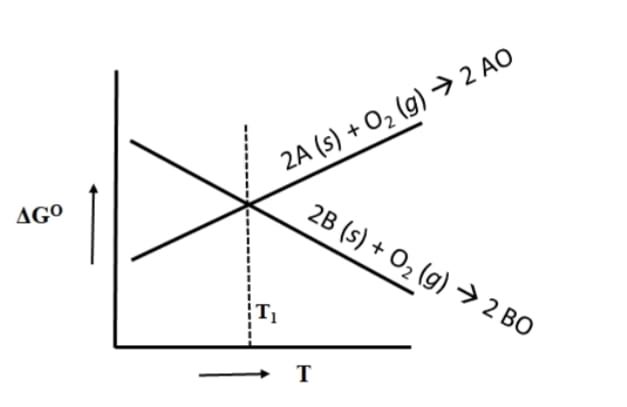
\includegraphics[width=0.6\textwidth]{images/qq6i.jpg}
\end{center}
\begin{enumerate}[label=(\alph*)]
    \item AO is a gas
    \item BO is a gas
    \item A will reduce BO above temperature $T_1$
    \item B will reduce AO below temperature $T_1$
\end{enumerate}

\item Terminal rise velocity of a spherical solid in a liquid obeys a relationship. According to Buckingham $\Pi$ theorem, the number of independent dimensionless variables needed to describe the phenomenon is \hspace{1em} (GATE 2019 MT)
\begin{enumerate}[label=(\alph*)]
    \item 1
    \item 2  
    \item 3   
    \item 5   
\end{enumerate}

\item Consider electrodeposition of copper on a copper electrode from an aqueous solution containing $0.5 \times 10^{-3}$ mol/cm$^3$ CuSO$_4$. The limiting current density (in mA/cm$^2$) is \hspace{1em} (GATE 2019 MT)
\begin{enumerate}[label=(\alph*)]
    \item 4.83
    \item 9.65  
    \item 19.30 
    \item 38.60
\end{enumerate}

\item The correct sequence of steelmaking operations is \hspace{1em} (GATE 2019 MT)  
[BOF: Basic Oxygen Furnace; LF: Ladle Furnace;  VD: Vacuum Degassing; CC: Continuous Casting]
\begin{enumerate}[label=(\alph*)]
    \item BOF $\to$ LF $\to$ VD $\to$ CC
    \item CC $\to$ BOF $\to$ LF $\to$ VD
    \item VD $\to$ CC $\to$ BOF $\to$ LF
    \item LF $\to$ BOF $\to$ VD $\to$ CC
\end{enumerate}

\item The common ore of titanium is \hspace{1em} (GATE 2019 MT)
\begin{enumerate}[label=(\alph*)]
    \item Bauxite
    \item Chalcopyrite
    \item Cassiterite
    \item Ilmenite
\end{enumerate}

\item Coarse suspended particles are to be separated from a flowing gas in a dust catcher. All factors remaining same, maximum gas-solid separation is expected from the dust catcher shown below. (GATE 2019 MT)
\begin{center}
    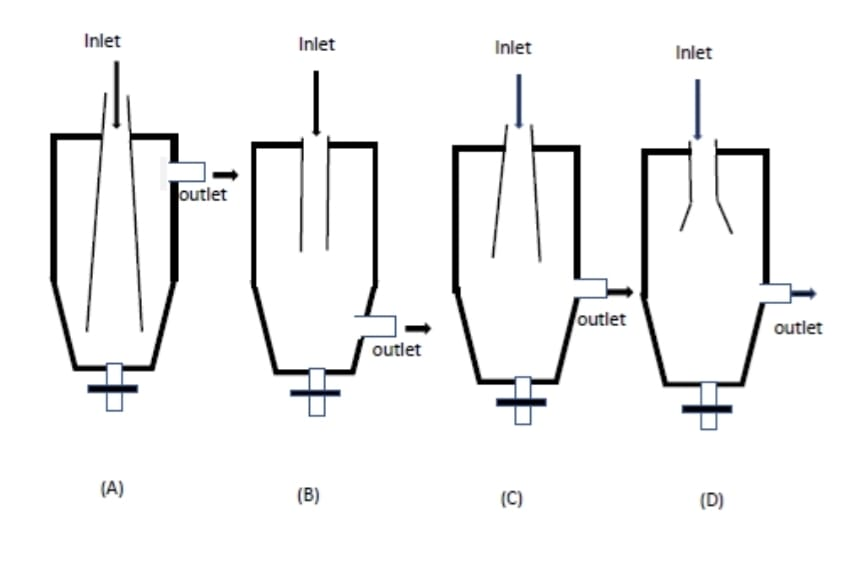
\includegraphics[width=0.9\textwidth]{images/qq11oi.jpg}
\end{center}

\item The Boudouard (carbon gasification) reaction is \hspace{1em} (GATE 2019 MT)
\begin{enumerate}[label=(\alph*)]
    \item $C(s) + \frac{1}{2} O_2(g) \to CO(g)$
    \item $C(s) + O_2(g) \to CO_2(g)$
    \item $C(s) + CO_2(g) \to 2 CO(g)$
    \item $2 CO(g) + O_2(g) \to 2 CO_2(g)$
\end{enumerate}

\item The fastest diffusing element in iron at 1100$\, ^\circ$C is \hspace{1em} (GATE 2019 MT)
\begin{enumerate}[label=(\alph*)]
    \item Ni
    \item Co
    \item Cr
    \item C
\end{enumerate}

\item Hydrogen bonds are stronger than \hspace{1em} (GATE 2019 MT)
\begin{enumerate}[label=(\alph*)]
    \item Ionic bonds
    \item Metallic bonds
    \item van der Waals bonds
    \item Covalent bonds
\end{enumerate}

\item The carbide primarily responsible for intergranular corrosion in austenitic stainless steel is \hspace{1em} (GATE 2019 MT)
\begin{enumerate}[label=(\alph*)]
    \item Cr$_{23}$C$_6$
    \item Fe$_3$C
    \item SiC
    \item Mn$_3$C
\end{enumerate}

\item During low strain rate ($\leq$ 0.1 sec$^{-1}$) deformation at room temperature, which metal deforms by twinning? (GATE 2019 MT)
\begin{enumerate}[label=(\alph*)]
    \item Fe
    \item Mg
    \item Al
    \item Ni
\end{enumerate}

\item In a tensile creep test, Nabarro-Herring mechanism is favored for \hspace{1em} (GATE 2019 MT)
\begin{enumerate}[label=(\alph*)]
    \item larger grain size and lower temperature
    \item smaller grain size and higher temperature
    \item larger grain size and higher temperature
    \item smaller grain size and lower temperature
\end{enumerate}

\item Beach marks are commonly observed on the fractured surfaces of metals after a \hspace{1em} (GATE 2019 MT)
\begin{enumerate}[label=(\alph*)]
    \item Creep test
    \item Fatigue test
    \item Impact test
    \item Compression test
\end{enumerate}

\item The length of internal cracks in two samples of the same glass is $c_1 = 0.5$ mm and $c_2 = 2$ mm. The ratio $(\sigma_1 / \sigma_2)$ of fracture strength is \hspace{1em} (GATE 2019 MT)
\begin{enumerate}[label=(\alph*)]
    \item 0.5
    \item 1.0
    \item 2.0
    \item 4.0
\end{enumerate}

\item Two blocks of the same metal are to be welded. The configuration that will undergo the least distortion after welding is \hspace{1em} (GATE 2019 MT)
\begin{center}
    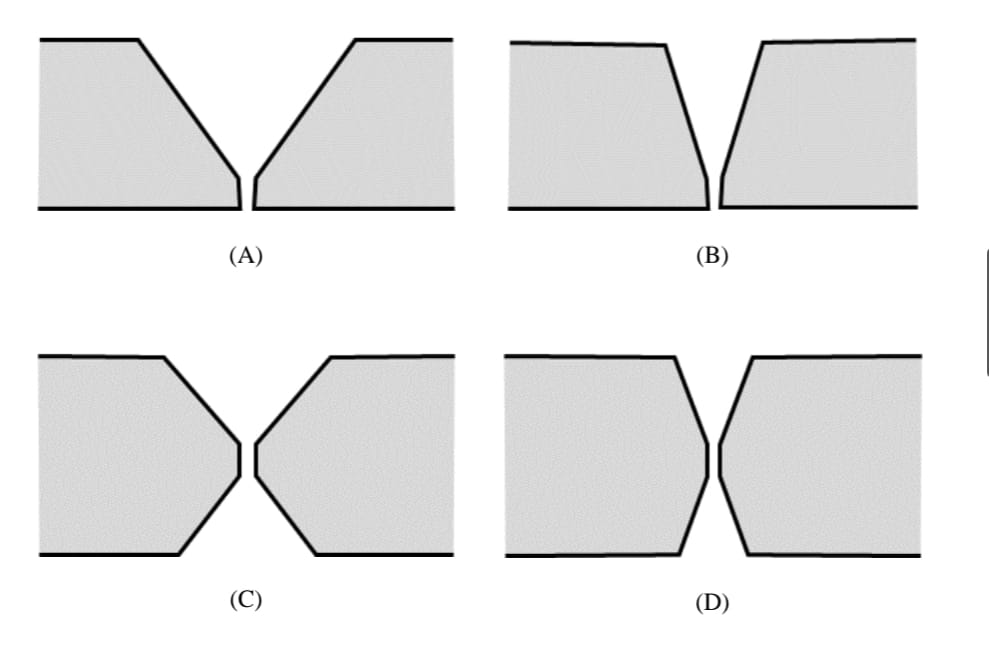
\includegraphics[width=0.9\textwidth]{images/qq20oi.jpg}
\end{center}

\item The most suitable non-destructive testing method for detecting small internal flaws in a dense bulk material is \hspace{1em} (GATE 2019 MT)
\begin{enumerate}[label=(\alph*)]
    \item Dye penetrant method
    \item Ultrasonic inspection
    \item Eddy current testing
    \item Magnetic particle inspection
\end{enumerate}

\item Alligatoring is a defect commonly observed in \hspace{1em} (GATE 2019 MT)
\begin{enumerate}[label=(\alph*)]
    \item Extrusion
    \item Deep drawing
    \item Sheet metal forming
    \item Rolling
\end{enumerate}

\item The standard deviation (rounded off to one decimal place) of the numbers $6, 8, 8, 9, 9$ is \hspace{1em} (GATE 2019 MT)
% NAT

\item An FCC crystal with lattice parameter 0.3615 nm is used to measure the wavelength of monochromatic X-rays. The Bragg angle ($\theta$) for the reflection from (111) planes is 21.68$^\circ$. The wavelength of X-rays (in nm, rounded to three decimals) is \hspace{1em} (GATE 2019 MT)


\item A plate of width 100 cm and thickness 5 cm is rolled to a thickness of 3 cm. If the entry velocity is 10 cm/s, what is the exit velocity (in cm/s, rounded to one decimal place)? Assume no change in plate width. (GATE 2019 MT)

















\item Match the reactors/refining sites in Column I with the corresponding refining processes in Column II. (GATE 2019 MT)
\begin{center}
\begin{tabular}{ll} 
Column I: Reactors / refining sites & Column II: Refining processes \\
(P) Blast furnace runner           & 1. De-carburization         \\
(Q) AOD                            & 2. External De-sulfurization   \\
(R) Torpedo car                    & 3. De-phosphorization      \\
(S) BOF                            & 4. External De-siliconization \\
\end{tabular}
\end{center}
\begin{enumerate}[label=(\alph*)]
    \item P-4, Q-1, R-2, S-3
    \item P-4, Q-2, R-3, S-1
    \item P-2, Q-1, R-4, S-3
    \item P-1, Q-3, R-2, S-4
\end{enumerate}

\item Match the injection metallurgy techniques in Column I with the corresponding objectives in Column II. (GATE 2019 MT)
\begin{center}
\begin{tabular}{ll}
Column I: Injection metallurgy techniques & Column II: Objectives \\
(P) Aluminium wire feeding    & 1. Inclusion modification \\
(Q) Calcium treatment         & 2. Mixing of liquid steel \\
(R) Argon rinsing             & 3. De-sulphurization \\
(S) Lime powder injection     & 4. Deoxidation \\
\end{tabular}
\end{center}
\begin{enumerate}[label=(\alph*)]
    \item P-2, Q-1, R-3, S-4
    \item P-4, Q-3, R-2, S-1
    \item P-3, Q-4, R-1, S-2
    \item P-4, Q-1, R-2, S-3
\end{enumerate}

\item The table providing correct information about crystal structure, coordination number and packing fraction is (GATE 2019 MT)
\begin{enumerate}[label=(\alph*)]
    \item \begin{tabular}{ccc} Crystal structure & CN & PF \\ FCC & 12 & 0.74 \\ BCC & 8 & 0.68 \\ DC & 4 & 0.34 \end{tabular}
    \item \begin{tabular}{ccc} Crystal structure & CN & PF \\ FCC & 8 & 0.74 \\ BCC & 4 & 0.68 \\ DC & 6 & 0.34 \end{tabular}
    \item \begin{tabular}{ccc} Crystal structure & CN & PF \\ FCC & 8 & 0.52 \\ BCC & 12 & 0.68 \\ DC & 12 & 0.74 \end{tabular}
    \item \begin{tabular}{ccc} Crystal structure & CN & PF \\ FCC & 12 & 0.74 \\ BCC & 8 & 0.68 \\ DC & 4 & 0.74 \end{tabular}
\end{enumerate}

\item Match the phase transformation in Column I with the corresponding reaction in Column II. (GATE 2019 MT)
\begin{center}
\begin{tabular}{ll}
Column I             & Column II              \\
(P) Peritectic        & 1. $\gamma \to \alpha + \beta$ \\
(Q) Monotectic        & 2. $L_1 + L_2 \to \alpha$ \\
(R) Eutectoid         & 3. $L_1 \to L_2 + \alpha$ \\
(S) Syntectic         & 4. $L + \alpha \to \beta$ \\
\end{tabular}
\end{center}
\begin{enumerate}[label=(\alph*)]
    \item P-4, Q-3, R-1, S-2
    \item P-3, Q-4, R-2, S-1
    \item P-1, Q-3, R-4, S-2
    \item P-4, Q-2, R-3, S-1
\end{enumerate}

\item In a typical scanning electron microscope (SEM) image, information about topography and atomic contrast are obtained from (GATE 2019 MT)
\begin{enumerate}[label=(\alph*)]
    \item secondary electron and auger electron, respectively
    \item primary electron and secondary electron, respectively
    \item secondary electron and back-scatter electron, respectively
    \item back-scatter electron and auger electron, respectively
\end{enumerate}

\item Match the ceramics in Column I with corresponding application in Column II. (GATE 2019 MT)
\begin{center}
\begin{tabular}{ll}
(P) Mullite          & 1. Cutting tools \\
(Q) Spinel ferrites  & 2. Refractories \\
(R) Tungsten carbide & 3. Piezoelectric \\
(S) Barium titanate  & 4. Soft magnet \\
\end{tabular}
\end{center}
\begin{enumerate}[label=(\alph*)]
    \item P-2, Q-3, R-1, S-4
    \item P-4, Q-1, R-2, S-3
    \item P-3, Q-4, R-1, S-2
    \item P-2, Q-4, R-1, S-3
\end{enumerate}

\item An aluminium single crystal is loaded in tension along [110] axis. Among the following slip systems, the one that will be activated first is (GATE 2019 MT)
\begin{enumerate}[label=(\alph*)]
    \item (111)[2]
    \item (111)
    \item (111)
    \item (111)[2]
\end{enumerate}

\item The correct Mohr’s circle construction for the stress state given below is (GATE 2019 MT)
% Options image
\begin{center}
    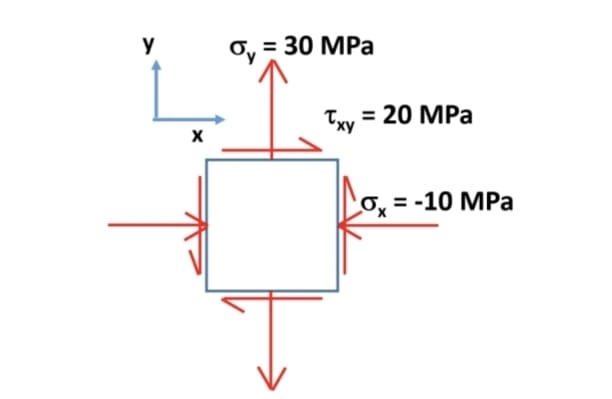
\includegraphics[width=0.95\textwidth]{images/qq33i.jpg}
\end{center}
Options:
\begin{center}
    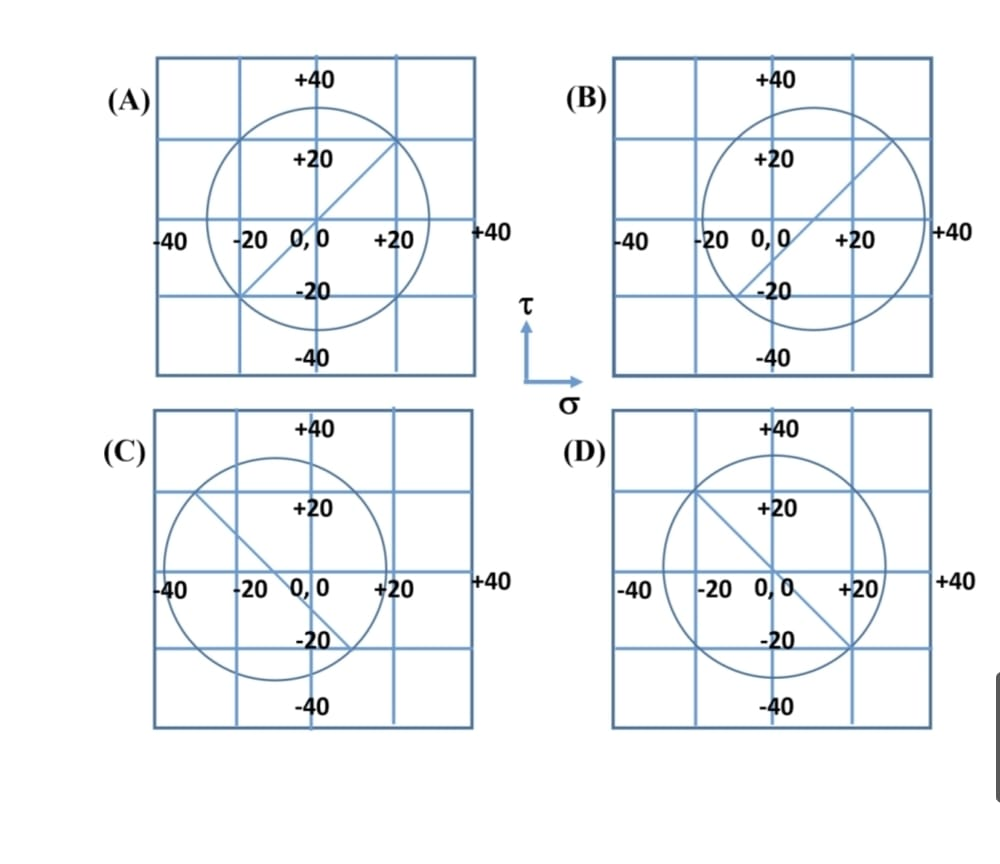
\includegraphics[width=0.95\textwidth]{images/qq33oi.jpg}
\end{center}

\item Match the automobile components in Column I with the corresponding manufacturing processes in Column II. (GATE 2019 MT)
\begin{center}
\begin{tabular}{ll}
(P) Engine block      & 1. Forging \\
(Q) Brake pad         & 2. Sheet metal forming \\
(R) Connecting rod    & 3. Casting \\
(S) Door panel        & 4. Powder metallurgy \\
\end{tabular}
\end{center}
\begin{enumerate}[label=(\alph*)]
    \item P-1, Q-2, R-3, S-4
    \item P-3, Q-4, R-1, S-2
    \item P-3, Q-2, R-4, S-1
    \item P-4, Q-1, R-3, S-2
\end{enumerate}

\item The equilibrium constant for the reaction at 300 K is
\[
\text{C(graphite) + 2 H}_2(g) \rightarrow \text{CH}_4(g)
\] 
Given: $\Delta H^\circ = -74,900$ J/mol, $\Delta S^\circ = -80$ J/mol K, $R = 8.314$ J/mol K. (GATE 2019 MT)
\begin{enumerate}[label=(\alph*)]
    \item $5.6 \times 10^6$
    \item $3.6 \times 10^7$
    \item $4.0 \times 10^8$
    \item $7.3 \times 10^8$
\end{enumerate}






















\item A 50 cm long rod is placed against a vertical wall such that the bottom of the rod is 30 cm away from the wall. If the bottom of the rod is pulled horizontally away from the wall at 4 cm/s, the top of the rod starts sliding down the wall with an instantaneous velocity (in cm/s, rounded off to two decimal places) of magnitude ________. (GATE 2019 MT)
% NAT

\item The probability of solving a problem by Student A is $1/3$, by Student B is $2/5$. The probability (rounded off to two decimal places) that at least one of the students solves the problem is ________. (GATE 2019 MT)
% NAT

\item Numerical value of work done (rounded off to the nearest integer) by a position-dependent force $\vec{F} = x\hat{i} + xy\hat{j}$ along the path $y = x^2$ from $(0,0)$ to $(2,4)$ in the $xy$ plane is ________. (GATE 2019 MT)
% NAT

\item The estimated value of the cube root of 37 (rounded off to two decimal places) obtained from the Newton-Raphson method after two iterations $x_2$ is ________ (starting with $x_0 = 1$). (GATE 2019 MT)
% NAT

\item The partial pressure of zinc (in torr, rounded off to two decimal places) in equilibrium with liquid lead containing $0.03$ mole $\%$ zinc at $900$ K is ________.
Given: Vapour pressure of pure zinc $(p^\circ_\text{Zn})$ at $900$ K is $0.027$ atm. Henry’s law coefficient $(\gamma^\circ_\text{Zn})$ for zinc at infinite dilute solution in lead on Raoultian scale is $8.55$. $1\text{ torr} = 1.316\times 10^{-3}$ atm. (GATE 2019 MT)
% NAT

\item Steady state radial heat conduction through a hollow, infinitely long zirconia cylinder is governed by the ODE: 
\[
\dfrac{1}{r}\dfrac{d}{dr}\left(r\dfrac{dT}{dr}\right)=0
\]
The inner surface of the cylinder is at $1473\,\text{K}$, the outer at $973\,\text{K}$. The rate of heat loss per unit length through the outer surface (in W/m, rounded off to nearest integer) is ________.
Given: Inner radius $= 0.05$ m; outer radius $= 0.07$ m; thermal conductivity of zirconia $k = 2$ W/m-K. (GATE 2019 MT)
% NAT

\item A $50$ mm (diameter) sphere of solid nickel is oxidized in a gas mixture containing $60\%$ argon and $40\%$ oxygen by volume. The rate of oxidation of nickel is controlled by oxygen transport through the concentration boundary layer. The rate of oxidation (in moles nickel per minute, rounded off to two decimal places) is ________.
Given: Total pressure $= 1$ atm; temperature $= 1173$ K; concentration of oxygen at surface $= 0$; boundary layer mass transfer coefficient $= 0.03$ m/s; $R = 8.205 \times 10^{-5}$ m$^3$ atm K$^{-1}$ mol$^{-1}$. Assume ideal gas behavior. (GATE 2019 MT)
% NAT

\item Equilibrium concentration of dissolved nitrogen (in wt.%, rounded off to three decimals) in pure liquid iron, exposed to atmospheric air at 1873 K, is ________.
Given: Sieverts’ law: $10\log K_N=[-1.063-518/T]$, with $K_N$ in atm$^{-1/2}$. (GATE 2019 MT)
% NAT

\item Pressure drop in the granular zone of a blast furnace is $300$ mm of water per meter of bed height. The bed permeability is $0.8$ m$^4$ N$^{-1}$ s$^{-1}$. The volumetric flow rate of gas per unit area through the bed [in (m$^3$.s$^{-1}$).m$^{-2}$, rounded off to the nearest integer] is ________.
Assume Darcy’s law and $g=9.8$ m/s$^2$, density of water $= 1000$ kg/m$^3$. (GATE 2019 MT)
% NAT

\item A blast furnace charged with hematite containing $90$ wt.\% Fe$_2$O$_3$ produces iron with $3.6$ wt.\% carbon. Coke ($90$ wt.\% C) is charged at $500$ kg per metric ton liquid iron. The blast furnace top gas contains (by volume), $22$\% CO, $18$\% CO$_2$, balance N$_2$. The volume of the blast furnace top gas (in m$^3$ NTP, rounded to nearest integer) is ________.
Given: Ideal gas; molar volume at NTP $= 22.4$ liter. (GATE 2019 MT)
% NAT

\item $100$ metric tons of copper concentrate containing $21$ wt.\% Cu is to be processed in 6 months with $25$ working days per month and $8$ hours per day. The concentrate is leached by sulphuric acid and electrolyzed in $10$ cells in series. The minimum current rating (Ampere per month per cell, rounded off to the nearest integer) is ________.
Given: Faraday constant $= 96500$ C/gram equivalent; atomic weight $= 63$. (GATE 2019 MT)
% NAT

\item Cold working of iron increases dislocation density from $10^{10}$ to $10^{15}$ m$^{-2}$. The stored energy (in MJ/m$^3$, rounded off to one decimal place) is ________.
Given: Shear modulus $= 82$ GPa, Burger’s vector $b = a_0[111]/2$, $a_0 = 0.2856$ nm. (GATE 2019 MT)
% NAT

\item The critical radius (in nm, rounded off to one decimal place) of nickel nucleus during solidification at $1673$ K is ________.
Given: Enthalpy of fusion $= 2.65\times 10^9$ J/m$^3$; interface energy $=0.5$ J/m$^2$; melting temp $=1728$ K. (GATE 2019 MT)
% NAT

\item A material made of alternating layers of A and B; 25\% volume B. If $E_A=200$ GPa, $E_B=100$ GPa$, $E_\text{material}$ (GPa, rounded to one decimal) is ________. (GATE 2019 MT)
% NAT

\item The S-N curve for a steel is shown. For stress ratio $(\sigma_{\min} / \sigma_{\max}) = -0.8$, the max stress (in MPa, rounded to nearest integer) for infinite fatigue life is ________.
\begin{center}
    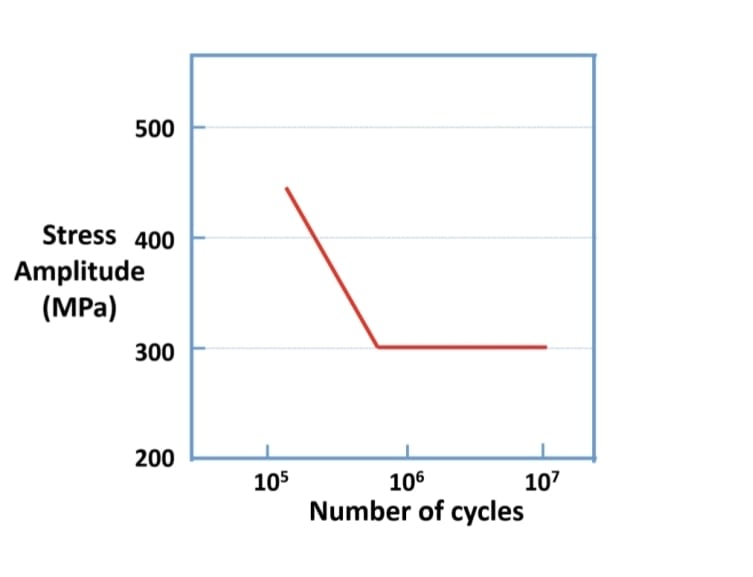
\includegraphics[width=0.9\textwidth]{images/qq50i.jpg}
\end{center}
% NAT

\item The true stress at necking (in MPa, rounded off to nearest integer) for $\sigma = 1750 \epsilon^{0.37}$ is ________. (GATE 2019 MT)
% NAT

\item In sand-mold casting, it takes $180$ s for complete solidification of a $27$ cm$^3$ cube. How long for a cylinder ($r=1$ cm, $h=6$ cm), all other conditions same? Total solidification time (in s, rounded to one decimal) is ________. (GATE 2019 MT)
% NAT

\item If solid-solid interfacial energy $(\gamma_{SS}) = 0.87$ J/m$^2$ and solid-liquid $(\gamma_{SL}) = 0.5$ J/m$^2$, the dihedral angle (degrees, rounded to one decimal) in sintering is ________. (GATE 2019 MT)
% NAT

\item The maximum possible reduction (in mm, rounded to one decimal) of a $100$ mm thick slab during rolling: coefficient of friction $=0.2$, roll diameter $=200$ mm. (GATE 2019 MT)
% NAT

\item An arc welding at $400$ A, $20$ V, speed $5$ mm/s, heat transfer efficiency $= 0.6$. The energy input per unit length (J/mm, rounded to nearest integer) is ________. (GATE 2019 MT)
% NAT

\end{enumerate}

















































\end{document}
